\section{\Dstar -meson systematics summary}

The summary for all systematics is shown in figure~\ref{fig:DstarSystSum}. The systematic uncertainties for this analysis are reported in Table~\ref{tab:Dstar_syst_summary}.


\begin{figure}[tb]
\begin{center}
 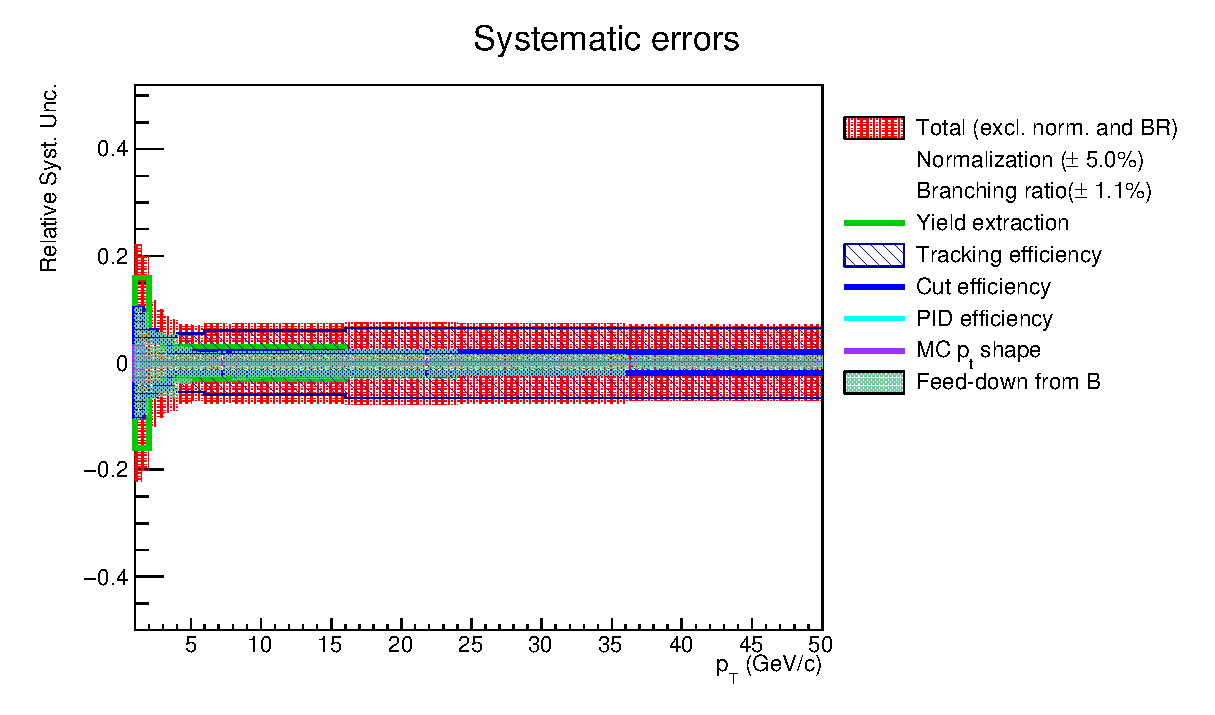
\includegraphics[width=1\textwidth]{figures/Dstar/pp13TeV/RelativeSystematics.eps}
\caption{Relative systematic uncertainties on the \pt -differential production cross section of prompt \Dstar.}
\label{fig:DstarSystSum}
\end{center}
\end{figure}


\begin{table}[htbp]
 \begin{center}
  \begin{tabular}{|c|c|c|c|c|c|c|c|c|c|c|c|}
\hline
\pt ($\GeV/c$) & 1-1.5 & 1.5-2 & 2-2.5 & 2.5-3 & 3-3.5 & 3.5-4 & 4-4.5 & 4.5-5 & 5-5.5 & 5.5-6 & 6-6.5 \\
\hline
Raw yeild & 10\% & 10\% & 5\% & 2\% & 2\% & 2\% & 2\% & 2\% & 2\%& 2\% & 2\% \\
\hline
Cut variations & 10\% & 6\% & 6\% & 4\% & 4\% & 2\% & 2\% & 2\% & 2\%& 2\% & 2\% \\
\hline
MC \pt -shape & 3\% & 0.5\% & 0\% & 0\% & 0\% & 0\% & 0\% & 0\% & 0\%& 0\% & 0\% \\
\hline
PID & 0\% & 0\% & 0\% & 0\% & 0\% & 0\% & 0\% & 0\% & 0\%& 0\% & 0\% \\
\hline
Tracking & 4.5\% & 4.5\% & 5\% & 5\% & 5\% & 5\% & 5.5\% & 5.5\% & 5.5\%& 5.5\% & 5.5\% \\
\hline
  \end{tabular}
 \end{center}

%\begin{table}[htbp]
 \begin{center}
  \begin{tabular}{|c|c|c|c|c|c|c|c|c|c|c|c|}
\hline
\pt ($\GeV/c$) & 6.5-7 & 7-7.5 & 7.5-8 & 8-9 & 9-10 & 10-12 & 12-16 & 16-24 & 24-36 & 36-50 \\
\hline
Raw yield & 2\% & 2\% & 2\% & 2\% & 2\%& 2\% & 2\% & 2\% & 2\% & 2\% \\
\hline
Cut variations & 2\% & 2\% & 2\% & 2\% & 2\%& 2\% & 2\% & 2\% & 2\% & 2\% \\
\hline
MC \pt -shape & 0\% & 0\% & 0\% & 0\% & 0\%& 0\% & 0\% & 0\% & 0\% & 0\% \\
\hline
PID & 0\% & 0\% & 0\% & 0\% & 0\%& 0\% & 0\% & 0\% & 0\% & 0\% \\
\hline
Tracking & 6\% & 6\% & 6\% & 6\% & 6\%& 6\% & 6\% & 6.5\% & 6.5\% & 6.5\% \\
\hline
  \end{tabular}
 \end{center}
 \caption{\Dstar systematic uncertainties summary.}
 \label{tab:Dstar_syst_summary}
\end{table} 

